\begin{figure}[H]
    \centering
    \fbox{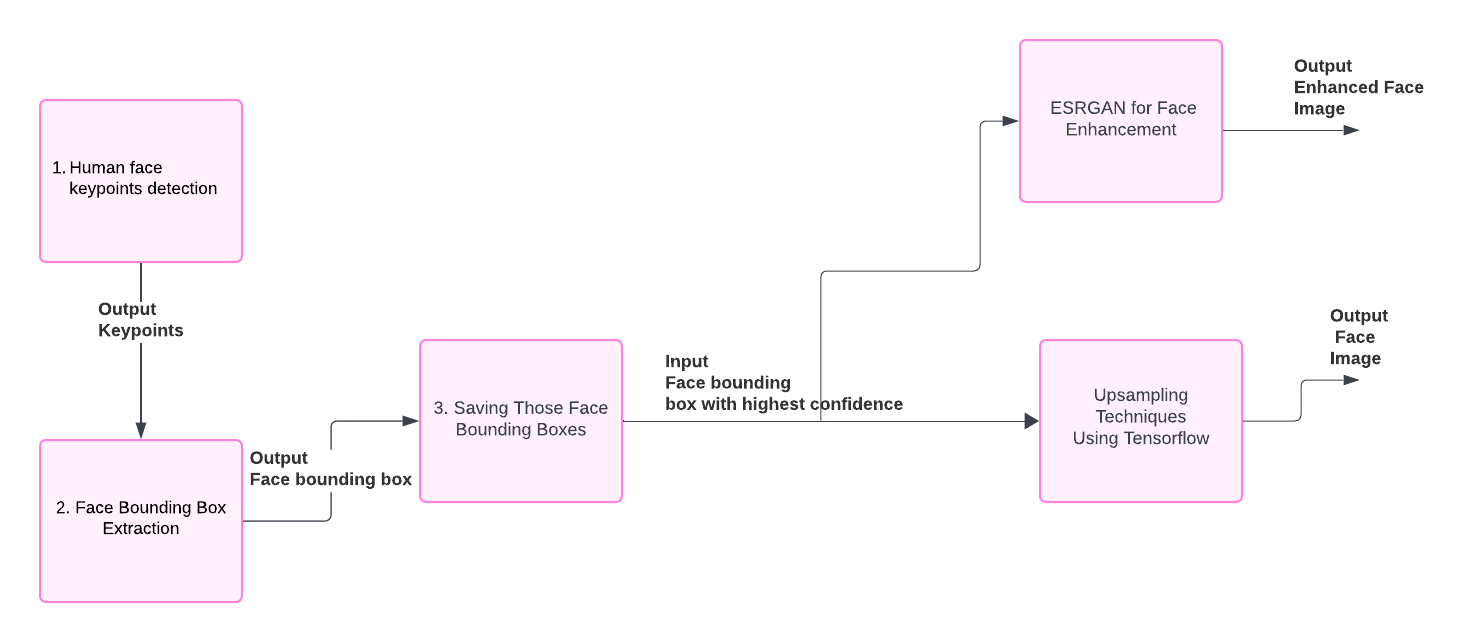
\includegraphics[width=\linewidth]{Flowdiagram Major project (1).png}}
    \caption{Flowchart}
    \label{fig:enter-label}
\end{figure}

\subsection{Face Extraction}
The face extraction process involves several steps, starting with keypoint detection using the YOLOv8 pose estimation model, followed by post-processing techniques to localize and extract the face bounding boxes accurately.

\subsubsection{Human Face keypoints Detection}

\begin{enumerate}
    \item The model takes an input of a video frame-wise and outputs a list of detection, each containing the estimated keypoints for a detected person. To handle multiple person scenarios, only the detection with the highest confidence score was considered.
    \item The model provides 17 keypoints for each detection, representing various body parts such as the nose, eyes, ears, shoulders, elbows, wrists, hips, knees, and ankles. The keypoints are represented as (x, y, confidence) tuples, where x and y denote the coordinates measured from the top-left corner of the image, and confidence indicates the detection confidence for that specific keypoint.
\end{enumerate}

\subsubsection{Face Bounding Box Extraction and Saving them}

\begin{enumerate}
    \item From the detected keypoints, the first five keypoints (nose, left eye, right eye, left ear, right ear) were considered for face bounding box extraction.
    \item The distance between the left eye and nose keypoints was calculated. If the left eye keypoint was not visible (i.e., coordinates were zero), the right eye keypoint was used instead.
    \item Based on a golden ratio of 1.5, i.e. height:width ratio, derived from anthropometric studies on the relationship between facial features, the width of the face bounding box was estimated as 2 times the distance between the eye and nose keypoints. Then calculating the height on the basis of golden ratio.
    \item Using the calculated width and the eye-nose distance, the top-left and bottom-right coordinates of the face bounding box were determined by subtracting and adding the width, respectively, from the eye and nose keypoint coordinates.
    \item The extracted face bounding boxes were cropped from the original video frames and saved as individual image files for further processing.
\end{enumerate}

This face extraction methodology leverages the accurate keypoint detection capabilities of the YOLOv8 model and applies geometric calculations based on anthropometric ratios to localize and extract face regions from video frames efficiently.

\subsection{Upsampling techniques}

Based on the information provided, here's an elaborated explanation of the upsampling techniques used in your methodology:

Upsampling Techniques

To enhance the resolution and visual quality of the extracted face bounding boxes, two different upsampling approaches were explored using TensorFlow's convolutional neural network (CNN) layers.

\textbf{Using TensorFlow Conv2DTranspose}

\begin{enumerate}
    \item The Conv2DTranspose layer in TensorFlow is designed for upsampling tensor inputs through a fractionally-strided convolution operation.
    \item A single Conv2DTranspose layer was used to upsample the input face bounding box images directly, without any additional preprocessing or resizing steps.
    \item The hyperparameters for the Conv2DTranspose layer were set as follows:\\
        - filters=1: Single output channel, as the input and output are grayscale images.\\
        - kernel-size=(8, 8)`: The size of the convolutional kernel used for upsampling.\\
        - `strides=(8, 8)`: The stride values determine the upsampling factor, effectively increasing the spatial dimensions of the input by a factor of 8 in both height and width.\\
        - `padding="valid"`: No padding was applied to the input tensor.\\
        - `activation=None`: No activation function was used, as the output represents the upsampled pixel values directly.\\
\end{enumerate}

The Conv2DTranspose layer provided a straightforward approach to upsampling the face bounding box images, but the results were not entirely satisfactory, as the upsampled images lacked fine details and exhibited blurring or artifacts.

\textbf{Using TensorFlow Upsampling and Conv2D}

\begin{enumerate}
    \item To improve the upsampling quality, a combination of TensorFlow's Upsampling layer and Conv2D layers was employed.
    \item The Upsampling layer was first used to increase the spatial dimensions of the input tensor.
    \item Following the upsampling operation, one or more Conv2D layers were applied to the upsampled tensor
\end{enumerate}

The combination of Upsampling and Conv2D layers yielded superior results compared to the Conv2DTranspose approach alone. The upsampled face bounding box images exhibited improved sharpness, reduced artifacts, and better preservation of facial features and details.

\subsection{ESRGAN for face enhancement}

Both upsampling techniques were limited in their ability to recover high-frequency details and textures, especially when applied to low-resolution or poor-quality face bounding boxes extracted from surveillance footage. To further enhance the visual quality, a more advanced super-resolution technique was explored using the ESRGAN model.\\

Using the tensorflow implementations for Image Super Resolution, we passed the image to their implementation for enhancement. 